\documentclass[12pt]{report}
\usepackage[utf8]{inputenc}
\usepackage[margin=1.2in]{geometry}
\usepackage{graphicx}
\usepackage{float}
\usepackage{subcaption}
\usepackage{amsmath}
\usepackage{amssymb}
\usepackage{ulem}
\usepackage{bm}
\usepackage{framed}
\usepackage{xcolor}
\usepackage{ragged2e}
\usepackage{color}
\usepackage{soul}
\graphicspath{ {images/} }
\setlength{\parskip}{1em}
\allowdisplaybreaks

\usepackage{titling}
\newcommand{\subtitle}[1]{%
	\posttitle{%
		\par\end{center}
	\begin{center}\large#1\end{center}
	\vskip0.5em}%
}

\newenvironment{blueframed}[1][blue]
{\def\FrameCommand{\fboxsep=\FrameSep\fcolorbox{#1}{white}}%
	\MakeFramed {\advance\hsize-\width \FrameRestore}}
{\endMakeFramed}

\newenvironment{spmatrix}[1]
{\def\mysubscript{#1}\mathop\bgroup\begin{bmatrix}}
	{\end{bmatrix}\egroup_{\textstyle\mathstrut\mysubscript}}

\title{Tutorial 5}
\subtitle
{
	\textbf{keywords}: estimators, unbiasedness, expected value, variance, multiple linear regression, interpretation, ceteris paribus, prediction, interpretation, R squared
	
	\textbf{estimated reading time}: 30 minutes
}
\author{Quang Bui}
\date{August 21, 2018}

\begin{document}
	
\maketitle

\newpage
\section*{Question 1}
$$(Discussed\ in\ class)$$

\newpage
\section*{Question 2}
\underline{Multiple linear regression model and interpreting coefficients}

\noindent EViews workfile: $hprice.wf1$
\begin{figure}[H]
	\centering
	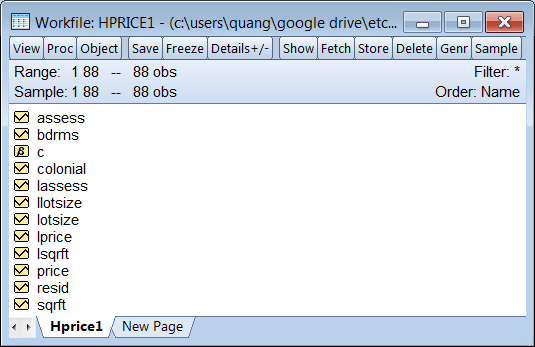
\includegraphics{q5_1}
\end{figure}
\vspace{-\baselineskip}
\noindent \textcolor{red}
{
	i. Estimate the model of $price$ on a constant, $sqrft$ and $bdrms$ and write out the results in equation form.
}
\noindent \textcolor{red}{$$price = \beta_0 + \beta_1sqrft + \beta_2bdrms + u$$ \begin{itemize}
		\item $price$ - house\ price\ (\$'000)
		\item $sqrft$ - area\ of\ the\ house\ (square foot)
		\item $bdrms$ - no.\ of\ bedrooms
\end{itemize}} \vspace{-\baselineskip}
$$Quick \to Estimate\ Equation$$
\begin{figure}[H]
	\centering
	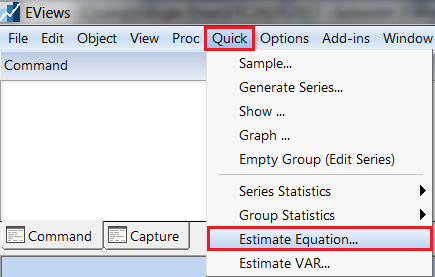
\includegraphics{q1_2}
\end{figure}
\vspace{-\baselineskip}
$$Equation\ Estimation: price\ c\ sqrft\ bdrms$$
\begin{figure}[H]
	\centering
	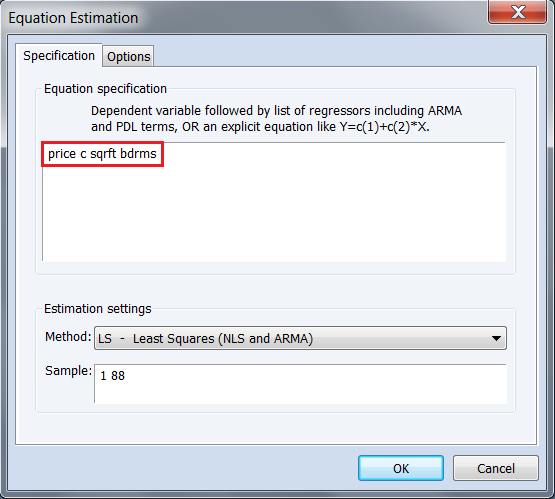
\includegraphics{q3_1}
\end{figure}
\vspace{-\baselineskip}
%%%%%%%%%% TABLE OBJECT %%%%%%%%%%
\begin{table}[H]
	\centering
	\begin{tabular}{lrrrr}
		\multicolumn{3}{l}{Dependent Variable: PRICE}&\multicolumn{1}{c}{}&\multicolumn{1}{c}{}\\
		\multicolumn{3}{l}{Method: Least Squares}&\multicolumn{1}{c}{}&\multicolumn{1}{c}{}\\
		\multicolumn{2}{l}{Sample: 1 88}&\multicolumn{1}{c}{}&\multicolumn{1}{c}{}&\multicolumn{1}{c}{}\\
		\multicolumn{3}{l}{Included observations: 88}&\multicolumn{1}{c}{}&\multicolumn{1}{c}{}\\
		[4.5pt] \hline \\ [-4.5pt]
		\multicolumn{1}{c}{Variable}&\multicolumn{1}{r}{Coefficient}&\multicolumn{1}{r}{Std. Error}&\multicolumn{1}{r}{t-Statistic}&\multicolumn{1}{r}{Prob.}\\
		[4.5pt] \hline \\ [-4.5pt]
		\multicolumn{1}{c}{C}&\multicolumn{1}{r}{$-19.31500$}&\multicolumn{1}{r}{$31.04662$}&\multicolumn{1}{r}{$-0.622129$}&\multicolumn{1}{r}{$0.5355$}\\
		\multicolumn{1}{c}{SQRFT}&\multicolumn{1}{r}{$0.128436$}&\multicolumn{1}{r}{$0.013824$}&\multicolumn{1}{r}{$9.290506$}&\multicolumn{1}{r}{$0.0000$}\\
		\multicolumn{1}{c}{BDRMS}&\multicolumn{1}{r}{$15.19819$}&\multicolumn{1}{r}{$9.483517$}&\multicolumn{1}{r}{$1.602590$}&\multicolumn{1}{r}{$0.1127$}\\
		[4.5pt] \hline \\ [-4.5pt]
		\multicolumn{1}{l}{R-squared}&\multicolumn{1}{r}{$0.631918$}&\multicolumn{2}{l}{Mean dependent var}&\multicolumn{1}{r}{$293.5460$}\\
		\multicolumn{1}{l}{Adjusted R-squared}&\multicolumn{1}{r}{$0.623258$}&\multicolumn{2}{l}{S.D. dependent var}&\multicolumn{1}{r}{$102.7134$}\\
		\multicolumn{1}{l}{S.E. of regression}&\multicolumn{1}{r}{$63.04484$}&\multicolumn{2}{l}{Akaike info criterion}&\multicolumn{1}{r}{$11.15907$}\\
		\multicolumn{1}{l}{Sum squared resid}&\multicolumn{1}{r}{$337845.4$}&\multicolumn{2}{l}{Schwarz criterion}&\multicolumn{1}{r}{$11.24352$}\\
		\multicolumn{1}{l}{Log likelihood}&\multicolumn{1}{r}{$-487.9989$}&\multicolumn{2}{l}{Hannan-Quinn criter.}&\multicolumn{1}{r}{$11.19309$}\\
		\multicolumn{1}{l}{F-statistic}&\multicolumn{1}{r}{$72.96353$}&\multicolumn{2}{l}{Durbin-Watson stat}&\multicolumn{1}{r}{$1.858074$}\\
		\multicolumn{1}{l}{Prob(F-statistic)}&\multicolumn{1}{r}{$0.000000$}&\multicolumn{1}{c}{}&\multicolumn{1}{c}{}&\multicolumn{1}{c}{}\\
		[4.5pt] \hline \\ [-4.5pt]
	\end{tabular}
	\caption{Regression output of $price$ on a constant, $sqrft$ and $bdrms$}
	\label{tbl:regout3}
\end{table}

\vspace{-\baselineskip}
\noindent When reporting the estimated model, we must not forget to include a `hat' above the dependent variable and $se(\hat{\beta}_j)$ underneath $\hat{\beta}_j$ in parenthesis,
\begin{align*}
	\widehat{price} &= \underset{(se(\hat{\beta}_0))}{\hat{\beta}_0} + \underset{(se(\hat{\beta}_1))}{\hat{\beta}_1}sqrft + \underset{(se(\hat{\beta}_2))}{\hat{\beta}_2}bdrms \\
	\widehat{price} &= -\underset{(31.0466)}{19.3150} + \underset{(0.0138)}{0.1284}sqrft + \underset{(9.4835)}{15.1982}bdrms
\end{align*}
\noindent \textcolor{red}
{
	ii. What is the estimated increase in price for a house with one more bedroom, holding square footage constant?
}
\newpage
\justify
\begin{blueframed}
\textcolor{blue}{\textbf{Background}}
\vspace{-\baselineskip}
\justify
\textcolor{blue}{\underline{Interpretation of estimated coefficients for multiple linear regression models}}

\noindent \textcolor{blue}
{
	\noindent Suppose we estimate a model of $y$ on a constant, $x_1$, and $x_2$,
	$$\hat{y} = \hat{\beta}_0 + \hat{\beta}_1x_1 + \hat{\beta}_2x_2$$
	if $x_1$ and $x_2$ changes by ${\Delta}x_1$ and ${\Delta}x_2$ respectively then,
	$$x_1\ becomes\ x_1 +{\Delta}x_1$$
	$$x_2\ becomes\ x_2 +{\Delta}x_2$$
	which will change $\hat{y}$,  
	$$\hat{y}\ becomes\ \hat{y}+{\Delta}\hat{y}$$
	This then gives us the following equation,
	\begin{align*}
		\hat{y}+{\Delta}\hat{y} &= \hat{\beta}_0 + \hat{\beta}_1(x_1 + {\Delta}x_1) + \hat{\beta}_2(x_2+{\Delta}x_2) \\
		&= \hat{\beta}_0 + \hat{\beta}_1x_1 + \hat{\beta}_2x_2 + \hat{\beta}_1{\Delta}x_1 + \hat{\beta}_2{\Delta}x_2 \\
		&= \hat{y} + \hat{\beta}_1{\Delta}x_1 + \hat{\beta}_2{\Delta}x_2 
	\end{align*}
	Since $\hat{y} = \hat{\beta}_0 + \hat{\beta}_1x_1 + \hat{\beta}_2x_2$, it must follow that,
	$${\Delta}\hat{y} = \hat{\beta}_1{\Delta}x_1 + \hat{\beta}_2{\Delta}x_2$$
	$\therefore$  the change in $\hat{y}$ for a 1-unit change in $x_1$, holding $x_2$ constant, is $\hat{\beta}_1$,
	$${\Delta}x_2 = 0$$
	$${\Delta}x_1 = 1$$
	\begin{align*}
		{\Delta}\hat{y} &= \hat{\beta}_1{\Delta}x_1 + \hat{\beta}_2{\Delta}x_2 \\
		&= \hat{\beta}_1\times 1 + \hat{\beta}_2\times 0 \\
		&= \hat{\beta}_1
	\end{align*}
	and the change in $\hat{y}$ for a 1-unit change in $x_2$, holding $x_1$ constant, is $\hat{\beta}_2$,
	$${\Delta}x_2 = 1$$
	$${\Delta}x_1 = 0$$
	\begin{align*}
	{\Delta}\hat{y} &= \hat{\beta}_1{\Delta}x_1 + \hat{\beta}_2{\Delta}x_2 \\
	&= \hat{\beta}_1\times 0 + \hat{\beta}_2\times 1 \\
	&= \hat{\beta}_2
	\end{align*}
	As we can see, $\hat{\beta}_1$ and $\hat{\beta}_2$ have a partial effect (ceteris paribus) interpretation!
}\end{blueframed}

\noindent From our estimated model, the changed in estimated house price depends on the change square footage and no. of bedrooms,
$$\Delta\widehat{price} = \hat{\beta}_1\Delta sqrft + \hat{\beta}_2\Delta bdrms$$
\noindent Note: The estimated intercept coefficient does not change the estimated house price.

\noindent If square footage is held constant,
$$\Delta sqrft = 0$$
\noindent then the change in the estimated house price depends only on the change in no. of bedrooms,
\begin{align*}
	\Delta\widehat{price} &= \hat{\beta}_1\Delta \times 0 + \hat{\beta}_2\Delta bdrms \\
	&= \hat{\beta}_2\Delta bdrms
\end{align*}
\noindent Therefore, the estimated increase in house price for for an additional bedroom, \uline{holding square footage constant},
\begin{align*}
\Delta\widehat{price} &= \hat{\beta}_2 \times 1 \\
&= 15.1982 \times 1 \\
&= 15.1982
\end{align*}
$$\$15,198.20$$
\noindent \textcolor{red}
{
	iii. What is the estimated increase in price for a house with an additional bedroom that is 140 square feet in size? Compare this to your answer in part (ii).
}
$$\Delta bdrms = 1$$
$$\Delta sqrft = 140$$
\begin{align*}
\Delta\widehat{price} &= \hat{\beta}_1\Delta sqrft + \hat{\beta}_2\Delta bdrms \\
&= 0.1284 \times 140+15.1982 \times 1 \\
&= 33.12
\end{align*}
$$\$33,120$$
\noindent The change in estimated house price is greater here than in ii) because we are also increasing the size of the house. In ii), we estimated the change in house price for an additional bedroom but kept the size of the house the same.

\noindent \textcolor{red}
{
	iv. What percentage of the variation in price is explained by square footage and number of bedrooms?
}
$$R^2 = 63.2\%$$
\noindent 63.2\% of the variation in house price is explained by square footage and number of bedrooms.

\noindent \textcolor{red}
{
	v. The first house in the sample has $sqrft=2438$ and $bdrms=4$. Find the predicted selling price for this house from the OLS regression line.
}
\begin{align*}
\widehat{price} &= -19.3150 + 0.1284sqrft + 15.1982bdrms \\
\widehat{price}_1 &= -19.3150 + 0.1284sqrft_1 + 15.1982bdrms_1 \\
&= -19.3150+0.1284 \times 2438+15.1982 \times 4 \\
&= 354.6052
\end{align*}
$$\$354,605$$
\noindent To perform this calculation in EViews,
$$Command\ Window: scalar\ prediction\ = c(1) + c(2)^{*}2438 + c(3)^{*}4$$
\begin{figure}[H]
	\centering
	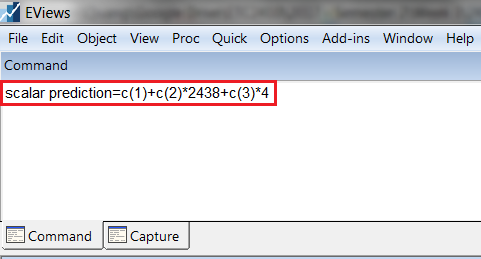
\includegraphics{q3_2}
\end{figure}
\vspace{-\baselineskip}
$$(press\ Enter\ to\ execute\ code)$$
\begin{figure}[H]
	\centering
	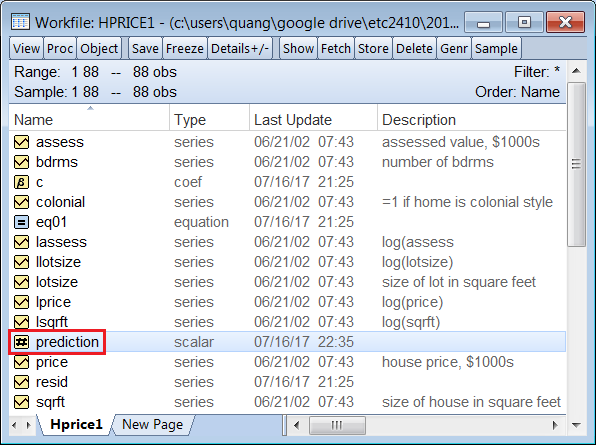
\includegraphics{q3_3}
\end{figure}
\vspace{-\baselineskip}
\begin{figure}[H]
	\centering
	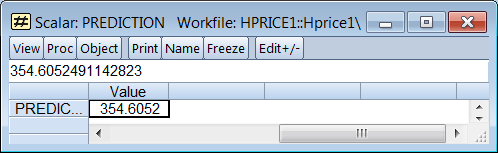
\includegraphics{q3_4}
\end{figure}

\noindent \textcolor{red}
{
	vi. The actual selling price of the first house in the sample was \$300,000 (so $price_1$=300). Find the residual for this house. Does it suggest that the buyer underpaid or overpaid for the house?
}
\begin{align*}
\hat{u}_i &= price_i - \widehat{price}_i \\
\hat{u}_1 &= price_1 - \widehat{price}_1 \\
&= 300 - 354.605 \\
&= -54.605
\end{align*}
$$-\$54,605$$
\noindent Based on our estimated model, the buyer underpaid, however, we have not considered other features that impact house price e.g. number of baths, age of house, whether it has been renovated etc.

\newpage
\section*{Question 3}
\noindent \textcolor{red}{We would like to make an ``app" where users input their easy to measure body characteristics and the app predicts their body fat percentage. We start with making an app for men. We have data on body fat percentage ($BODY\_FAT$), weight in kg ($WKG$) and abdomen circumference in cm ($ABDOMEN$) for 251 adult men. The matrix of scatter plots of each pair of these three variables in our sample is given below.}
\begin{figure}[H]
	\centering
	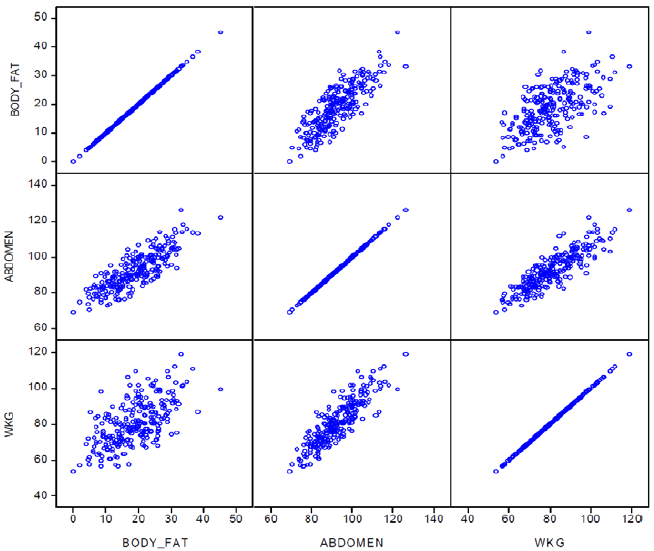
\includegraphics{tute5_28}
\end{figure}
\noindent \textcolor{red}{The plots in the first row are: the scatter plot of $body\ fat$ against $body\ fat$ (which is the 45 degree line) at the left corner, the scatter plot of body fat against abdomen circumference in the middle, and the scatter plot of body fat against weight in the top right corner. You can create these matrices in EViews by graphing more than 2 variables and them choosing scatter plot $$Quick \to Graph \to Scatter \to Multiple\ Series: Scatterplot\ Matrix$$ Without estimating any regressions, explain what these plots can tell us about each of the following (the correct answer for one of these is ``nothing"):}


\justify
\begin{blueframed}
	\textcolor{blue}{\textbf{Background}}
	\vspace{-\baselineskip}
	\justify
	\textcolor{blue}{\underline{OLS estimator for a simple linear regression model}}
	
	\noindent \textcolor{blue}
	{
		\noindent For the following simple linear regression model, $$y = \beta_0 + \beta_1 x_1 + u$$  the OLS estimator of $\beta_0$ and $\beta_1$ can be expressed by the following formulas,
		\begin{align*}
		\hat{\beta}_0 &= \bar{y} - \hat{\beta}_1\bar{x}_1 \\
		\hat{\beta}_1 &= \dfrac{\widehat{Cov(y,x_1)}}{\widehat{Var(x_1)}}
		\end{align*}
		or in matrix notation, $$\widehat{\boldsymbol{\beta}} 
		= (\textit{\textbf{X}}'\textit{\textbf{X}})^{-1}\textit{\textbf{X}}'\textit{\textbf{y}}
		=
		\begin{bmatrix}
		\hat{\beta}_0 \\
		\hat{\beta}_1 
		\end{bmatrix}
		=
		\begin{bmatrix}
		\bar{y} - \hat{\beta}_1\bar{x}_1 \\[10pt]
		\dfrac{\widehat{Cov(y,x_1)}}{\widehat{Var(x_1)}} 
		\end{bmatrix}$$
		since $\widehat{Var(x_1)}>0$, the sign of $\hat{\beta}_1$ depends directly on the sign of $\widehat{Cov(y,x_1)}$. \\ \\ For the multiple linear regression model, $$y = \beta_0 + \beta_1 x_1 + \beta_2 x_2 + \dots + \beta_k x_k + u$$ the OLS estimator of $\beta_1$ is not equal to $\dfrac{\widehat{Cov(y,x_1)}}{\widehat{Var(x_1)}}$, $$\hat{\beta}_1 \neq \dfrac{\widehat{Cov(y,x_1)}}{\widehat{Var(x_1)}}$$ $\therefore$ the sign of $\hat{\beta}_1$, in the estimated multiple linear regression model, does not depend directly on the sign of $\widehat{Cov(y,x_1)}$.
}\end{blueframed}

\noindent \textcolor{red}{(a) the sign of the coefficient of $ABDOMEN$ in a regression of $BODY\_FAT$ on a constant and $ABDOMEN$}
\begin{align*}
	BODY\_FAT &= \beta_0 + \beta_1 ABDOMEN + u \\
	\widehat{BODY\_FAT} &= \hat{\beta}_0 + \hat{\beta}_1 ABDOMEN
\end{align*}
\noindent For the simple regression model of $BODY\_FAT$ on a constant and $ABDOMEN$ the OLS estimator of $\beta_0$ and $\beta_1$ are given by the following formulas,
\begin{align*}
	\hat{\beta}_0 &= \overline{BODY\_FAT} - \hat{\beta}_1\overline{ABDOMEN} \\
	\hat{\beta}_1 &= \dfrac{\widehat{Cov(BODY\_FAT,ABDOMEN)}}{\widehat{Var(ABDOMEN)}}
\end{align*}
\noindent From the scatter plot, we can see that $BODY\_FAT$ and $ABDOMEN$ have a positive linear relationship, 
\begin{align*}
	&\therefore \widehat{Cov(BODY\_FAT,ABDOMEN)}>0 \\
	&\implies \hat{\beta}_1 > 0
\end{align*}

\noindent \textcolor{red}{(b) the sign of the coefficient of $WKG$ in a regression of $BODY\_FAT$ on a constant and $WKG$}$$(different\ model\ so\ I'm\ using\ a\ different\ Greek\ letter)$$
\begin{align*}
BODY\_FAT &= \alpha_0 + \alpha_1 WKG + u \\
\widehat{BODY\_FAT} &= \hat{\alpha}_0 + \hat{\alpha}_1 WKG
\end{align*}
\noindent For the simple regression model of $BODY\_FAT$ on a constant and $WKG$ the OLS estimator of $\alpha_0$ and $\alpha_1$ are given by the following formulas,
\begin{align*}
\hat{\alpha}_0 &= \overline{BODY\_FAT} - \hat{\alpha}_1\overline{WKG} \\
\hat{\alpha}_1 &= \dfrac{\widehat{Cov(BODY\_FAT,WKG)}}{\widehat{Var(WKG)}}
\end{align*}
\noindent From the scatter plot, we can see that $BODY\_FAT$ and $WKG$ have a positive linear relationship, 
\begin{align*}
&\therefore \widehat{Cov(BODY\_FAT,WKG)}>0 \\
&\implies \hat{\alpha}_1 > 0
\end{align*}

\noindent \textcolor{red}{(c) which of the two regressions explained in parts (a) and (b) is likely to have a better fit?} 
\begin{align}
\widehat{BODY\_FAT} &= \hat{\beta}_0 + \hat{\beta}_1 ABDOMEN \\
\widehat{BODY\_FAT} &= \hat{\alpha}_0 + \hat{\alpha}_1 WKG
\end{align}

\noindent The first estimated model is likely to fit the data better than the second. Why?

\noindent $R^2$, which is a measure of the models goodness of fit with the data is given by the formula, $$R^2 = 1 - \dfrac{SSR}{SST}$$ where \begin{itemize}
	\item $SSR$ - sum of squared residual $$SSR = \sum_{i=1}^{n}(BODY\_FAT_i - \widehat{BODY\_FAT}) = \sum_{i=1}^{n}\hat{u}^2_i$$
	\item $SST$ - sum of squared total $$SST = \sum_{i=1}^{n}(BODY\_FAT_i - \overline{BODY\_FAT})$$
\end{itemize}

\noindent From the scatter plot of $BODY\_FAT$ against $WKG$, an OLS regression line of $(1)$ through the scatter plot of $BODY\_FAT$ against $ABDOMEN$ would have a smaller $SSR$ than the OLS regression line of  $(2)$, $$SSR_{(1)} < SSR_{(2)}$$
\noindent Since $SST$ depends only on $body\ fat$ and sample mean of $body\ fat$ it is the same for both estimated models, $$SST_{(1)} = SST_{(2)} = SST$$ then the $R^2$ of $(1)$ will be higher than the $R^2$ of $(2)$, $$R^2_{(1)} = 1 - \dfrac{SSR_{(1)}}{SST} > R^2_{(2)} = 1 - \dfrac{SSR_{(2)}}{SST}$$

\noindent In the scatter plot of $BODY\_FAT$ against $ABDOMEN$, $BODY\_FAT$ is less dispersed around $\overline{BODY\_FAT}$ for each value of $ABDOMEN$ than it is for $WKG$. (Think about $R^2$.)

\noindent \textcolor{red}{(d) the sign of the coefficient of $WKG$ in a regression of $BODY\_FAT$ on a constant, $ABDOMEN$ and $WKG$.} $$BODY\_FAT = \beta_0 + \beta_1 ABDOMEN + \beta_2 WKG + u$$

\noindent Scatter plots cannot tell us anything about the correlation of body fat and weight \uline{after controlling for the influence of abdomen circumference}. So even though the scatter plot tells us that body fat and weight have a positive linear relationship, $$\widehat{Cov}(BODY\_FAT,WKG) > 0$$ we do not know whether weight still has positive impact body fat after controlling for abdomen circumference.

\noindent (In fact, it actually has a negative impact after controlling for abdomen circumference! Think about 2 people with the same abdomen circumference i.e. controlling for $ABDOMEN$, but one weights more than the other. Since both have the same abdomen circumference, the one that is heavier will have weight distributed elsewhere in his body e.g. broader shoulders, thicker quads, fuller chest etc. If both males have the same abdomen circumference, the one with the bigger shoulders, quads, chest, etc. is likely to have a better physique and quite likely less body fat.)

\newpage
\section*{Question 4 }
\noindent EViews workfile: \textit{bodyfat.wf1}

\noindent \textcolor{red}{With the same data as above, we have estimated three regressions: \begin{align*}
		\widehat{BODY\_FAT} &= -12.63 + 0.39WKG, \qquad R^2 = 0.385, \bar{R}^2 = 0.382 \\
		\widehat{BODY\_FAT} &= -38.60 + 0.62ABDOMEN, \qquad R^2 = 0.681, \bar{R}^2 = 0.679 \\
		\widehat{BODY\_FAT} &= -42.94 + 0.91ABDOMEN - 0.27WKG, \qquad R^2 = 0.724, \bar{R}^2 = 0.722
	\end{align*}}

\noindent \textcolor{red}{(a) The signs of the $R^2$s of the first two regressions must agree with your answers to parts (a), (b), and (c) of the previous question. If they don't then discuss these in the tutorial or during consultation} $$They\ do!$$

\noindent \textcolor{red}{(b)} $$(Discussed\ in\ Question\ 3(d))$$

\noindent \textcolor{red}{(c) If weight was measured in pounds regard than kilograms (each kilogram is 2.2 pounds), how would the above regression results change? Check your answers by running the regressions using $bodyfat.wf1$ file.} \begin{align*}
	WEIGHTLB &= 2.2\times WKG \\
	WKG &= \dfrac{WEIGHTLB}{2.2}  
\end{align*} 
\begin{align*}
	\widehat{BODY\_FAT} &= -12.63 + 0.39WKG \\
	&= -12.63 + \dfrac{0.39}{2.2}WEIGHTLB \\
	&= -12.63 + 0.177WEIGHTLB
\end{align*} So we should find that when regressing body fat on a constant and weight in pounds, the estimated coefficient of weight in pounds equals to the estimated coefficient of weight in kg divided by $2.2$ $$\dfrac{0.39}{2.2} = 0.177$$ The $R^2$ and other estimated coefficients stay the same.

\noindent Since weight in pounds equals to weight in kg times 2.2, a regression of body fat on a constant and weight in pounds is given by, $$BODY\_FAT = \beta_0 + \beta_1 WKG^*2.2 + u$$ which gives the followed estimated regression model,
\begin{figure}[H]
	\centerline{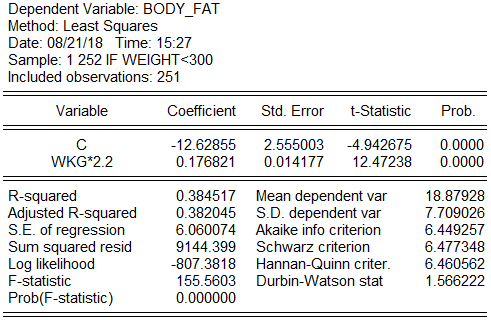
\includegraphics{q4_5}}
\end{figure}
\vspace{-\baselineskip} $$\widehat{BODY\_FAT} = -\underset{(2.5550)}{12.63} + \underset{(0.0142)}{0.1768} WKG$$

\noindent \textcolor{red}{(d) If body fat was regressed on a constant only, what would the OLS estimate of the constant be? Answer it first and then check your answer using $bodyfat.wf1$ file.} $$BODY\_FAT = \beta_0 + u$$ 
\noindent Since the regression model has only one parameter to estimate, $$\beta_0$$ the OLS formula gives an estimate of $\beta_0$,
$$\widehat{\boldsymbol{\beta}} 
= (\textbf{X}'\textbf{X})^{-1}\textbf{X}'\textbf{y}
=
\hat{\beta}_0$$
$$
\textbf{X}'\textbf{X}= 
\begin{spmatrix}{1 \times n}
	1 & 1 & \cdots & 1
\end{spmatrix}
\begin{spmatrix}{n \times 1}
	1 \\
	1 \\
	\vdots \\
	1 
\end{spmatrix}
= n
$$
$$\therefore (\textbf{X}'\textbf{X})^{-1}= \dfrac{1}{n}$$
$$\textbf{X}'\textbf{y} = 
\begin{spmatrix}{1 \times n}
1 & 1 & \cdots & 1
\end{spmatrix}
\begin{spmatrix}{n \times 1}
BODY\_FAT_1 \\
BODY\_FAT_2 \\
\vdots \\
BODY\_FAT_n
\end{spmatrix}
= \sum_{i=1}^{n}BODY\_FAT_i$$
\begin{align*}
	\therefore \widehat{\boldsymbol{\beta}} 
	&= (\textbf{X}'\textbf{X})^{-1}\textbf{X}'\textbf{y} \\
	&= \dfrac{1}{n}\sum_{i=1}^{n}BODY\_FAT_i \\
	&= \overline{BODY\_FAT} \\
	&=\hat{\beta}_0
\end{align*}
\begin{figure}[H]
	\centerline{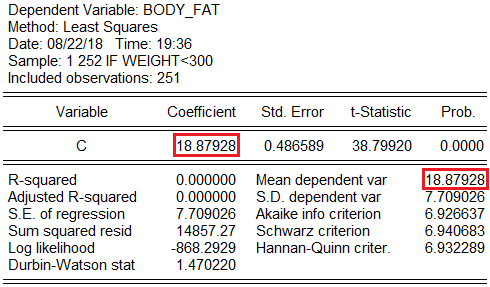
\includegraphics{q4_6}}
\end{figure}


\end{document}
